\section{数值例证}
\subsection{精确反馈的二维算例}
本节以两个二维模型和一组预先规定的标量实验核验理论机制。
二维模型为
\[
{\bm{A}}_{\rm S}=\begin{bmatrix}.82&.18\\-.10&.72\end{bmatrix},\qquad
{\bm{A}}_{\rm U}=\begin{bmatrix}1.04&.12\\.03&.91\end{bmatrix},
\]
\[
{\bm{P}}_0=\begin{bmatrix}.8&.12\\.12&.6\end{bmatrix},\quad
{\bm{Q}}=\begin{bmatrix}.05&.01\\.01&.04\end{bmatrix},\quad
{\bm{R}}=\begin{bmatrix}.2&.03\\.03&.3\end{bmatrix},\quad
{\bm{Z}}=\begin{bmatrix}2&.25\\.25&1.5\end{bmatrix}.
\]
目标$k=4$、$b=0.1$。计算考察持续定向策略，以及目标拍随机符号、下一拍补偿的两拍策略。
定理下界采用单拍构造；此处两拍策略作为另一条合法数值见证报告，
不将其数值常数用于单拍证明。

\begin{table}[ht]
\centering\footnotesize
\bicaption{真实目标损伤分解（精确反馈）}{Table \thetable\quad Decomposition of target damage under exact feedback}
\begin{tabular}{llrrr}
\toprule
Model & Policy & Bias energy & Covariance change & Damage $J$\\
\midrule
S & Persistent direction & .001315759 & -.000020445 & .001295314\\
U & Persistent direction & .003252364 & -.000120021 & .003132343\\
S & Two-step sign compensation & .000321850 & 0 & .000321850\\
U & Two-step sign compensation & .000573797 & 0 & .000573797\\
\bottomrule
\end{tabular}
\end{table}
持续策略的协方差变化为负，说明只报告条件偏差平方会高估这些例子的真实损伤。
原两拍策略在目标之前无动作，目标协方差分布不变，所以该项为零。
各组合使用事件树计算；另在$b=0.2$下，对两个模型和两种策略分别以40万次独立重置结果交叉检查。

\begin{table}[ht]
\centering\footnotesize
\bicaption{两拍符号补偿策略的损伤及不同保证（$b=0.1$）}{Table \thetable\quad Damage and distinct guarantees for the two-step sign-compensation policy}
\begin{tabular}{lrr}
\toprule
Quantity & S & U\\
\midrule
True damage & .000321850 & .000573797\\
Population certificate & .000457526 & .000902386\\
Certificate / damage & 1.42155 & 1.57266\\
Upper / witness lower bound (TV-linear region) & 783.639 & 359.136\\
$N=10^4$: mean-centered confidence bound, known reference & .084711 & .072733\\
\bottomrule
\end{tabular}
\end{table}
最后一行按Hoeffding不等式计算，并将经验均值置于总体均值，
不是新采样所得认证结果。总体证书在这两个例子中较接近真实损伤，
有限样本余量却仍很大。双预算曲线只是全策略上界与一条合法构造下界，
不代表真实最优值已经被数值求解。原事件串TV也不替代完整连续日志TV；
后者预算可行性由解析联合核界提供。

\subsection{预先规定的标量验证}
量化扩展仅在标量范围验证。S1/U1取$A=0.82/1.04$，
$m_0=0$、$P_0=0.8$、$Q=0.05$、$R=0.2$、$Z=2$，目标$k=4$，$b=b_{\rm ref}=0.1$。
这些是由旧参数首坐标系数构成的独立标量模型，删除耦合后不等于原二维系统的边缘。
每模型使用预先固定的2048条独立基础物理与触发样本，
在三个精度、A/B协议及健康/正/负分支之间共享样本。
两符号分支取平均以评价等概率符号策略，统计独立单位仍是基础样本。
总共4096个模型内独立样本，73728条短方法分支，各运行至$k+1$事件；
C和A-rounded-log只是现有轨迹的观察字段，没有额外状态递推。

量化精度由固定协方差常数选定：
\[
\delta_{\rm cap}=\min\{0.1,\delta_*/2,\alpha_{\max}b/2\},\qquad
\delta_j=\delta_{\rm cap}\{1/4,1/2,1\},\quad
\eta_j=\delta_j/(2\alpha_{\max}).
\]
参数选择先于随机输入产生，精度列表见表\ref{tab:e1-damage}。
A的$\delta$仅为共同门控和剂量标签，不改变精确触发中心；
B采用实际量化反馈和一致静默更新。
二者分别用自己的合法历史决定目标拍中央格门控，不能调用另一协议的健康反事实。
所有动作在真实发送之后发生，其他时刻无动作。
这里比较的是同形式合法见证，不要求A/B的实际动作概率、能量或通信率完全相等。

独立重算核对了事件时序、健康条件均值、量化码及损伤恒等式。
配对损伤与$K_h^2\eta^2\ind_E$的最大绝对差为$3.66\times10^{-16}$。
以下95\%区间来自1000次按基础样本的配对bootstrap，是见证损伤的探索性区间，不是全策略安全置信界。

\begin{table}[ht]
\centering\footnotesize
\bicaption{B协议的见证损伤：精度主导区域}{Table \thetable\quad Feasible witness damage under B in the precision-dominated regime}
\label{tab:e1-damage}
\begin{tabular}{lrrrr}
\toprule
Model / level & $\delta$ & $10^6\hat J$ & Exploratory 95\% interval ($\times10^6$) & $\hat J/\delta^2$\\
\midrule
S1/1 & .00290706 & .295503 & [.256237,.334963] & .034967\\
S1/2 & .00581412 & 1.239223 & [1.086202,1.391006] & .036659\\
S1/3 & .01162823 & 4.814492 & [4.227691,5.429128] & .035606\\
U1/1 & .00556494 & .785686 & [.703663,.878413] & .025370\\
U1/2 & .01112988 & 2.793531 & [2.458229,3.128096] & .022551\\
U1/3 & .02225976 & 11.211802 & [9.942383,12.533812] & .022627\\
\bottomrule
\end{tabular}
\end{table}
各点均为所构造攻击见证的可达到损伤，而非最坏值$V$的数值求解。
本设计令$\eta$随$\delta$变化且均远小于$b$，只考察精度主导区；
不能据三个点声称数值验证了$\min\{b^2,\delta^2\}$的两个区域或估计出一般渐近指数。
A同剂量的见证损伤在S1中为$2.92\times10^{-7}$至$4.81\times10^{-6}$，
在U1中为$7.76\times10^{-7}$至$1.08\times10^{-5}$，详图\ref{fig:e1}。

\begin{figure}[ht]
\centering
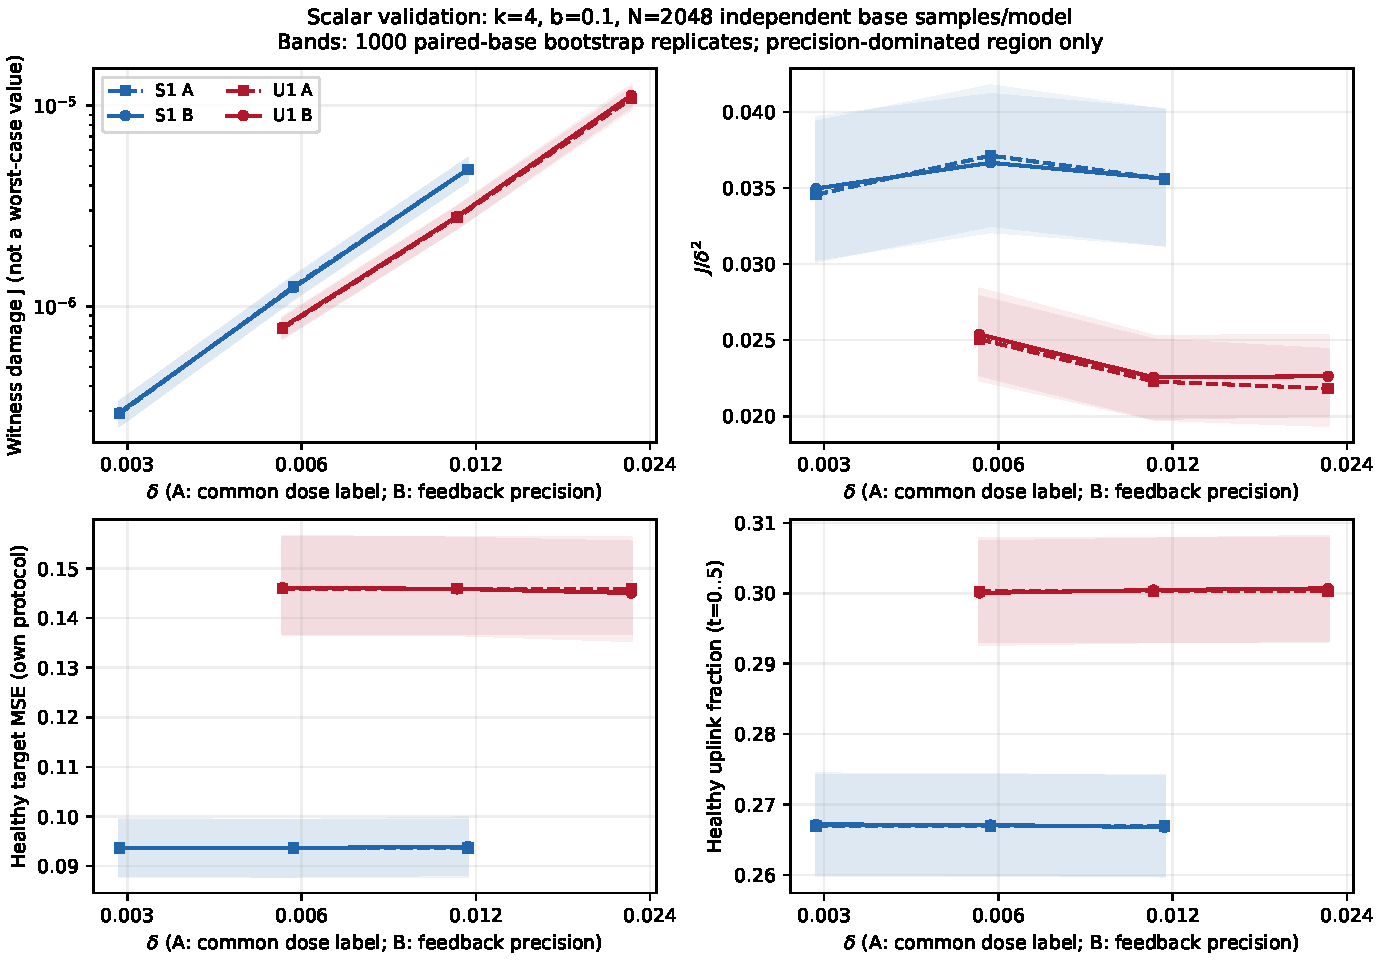
\includegraphics[width=\linewidth]{figures/e1_mechanism.pdf}
\bicaption{标量见证损伤、精度尺度及健康代价；阴影为基础样本配对bootstrap区间}
{Fig. \thefigure\quad Scalar witness damage, precision scaling, and healthy cost.
Shading denotes paired bootstrap intervals. For A, $\delta$ is a dose label; for B, it is the actual feedback precision.}
\label{fig:e1}
\end{figure}

\subsection{各自健康基线及可信记录的一致性}
A的健康MSE在S1/U1分别为0.093640886、0.145956498，
0--5拍平均上行发送率分别为0.266927、0.300293，且不依测试剂量改变。
B各精度结果见表\ref{tab:e1-health}。受攻MSE从相应B健康基线增加，
未把量化本身的健康差异计入攻击损伤。
健康B减A的MSE探索区间在六组中均跨零，点估计有正有负，
不足以主张正常精度或通信收益。
在最大预设精度下，见证损伤约为对应B健康MSE的$0.0051\%$（S1）和$0.0077\%$（U1）。
该量级说明这里验证的是严格正损伤及其精度尺度，不支持“量化导致显著工程损害”的表述。

\begin{table}[ht]
\centering\footnotesize
\bicaption{B的健康和受攻MSE、通信及动作频次}{Table \thetable\quad Healthy and attacked MSE, transmission rate, and attack counts under B}
\label{tab:e1-health}
\begin{tabular}{lrrrr}
\toprule
Model / level & Healthy MSE & Attacked MSE & Healthy Tx rate & Attacks / 2048\\
\midrule
S1/1 & .093701541 & .093701837 & .267171 & 223\\
S1/2 & .093635897 & .093637136 & .267090 & 232\\
S1/3 & .093878253 & .093883067 & .266764 & 225\\
U1/1 & .146129290 & .146130075 & .300049 & 282\\
U1/2 & .145905461 & .145908255 & .300456 & 252\\
U1/3 & .145071599 & .145082811 & .300700 & 252\\
\bottomrule
\end{tabular}
\end{table}
B的健康与两符号运行在所有预定样本中均具有完全相同的事件、量化码和目标P，
与理论逐路径不变性一致；这一抽样检查不代替总体同律的证明。
实际幅值S1依次为0.00442673、0.00885346、0.01770692，
U1为0.00460144、0.00920288、0.01840576。
B的平均动作能量分别为S1的$2.13\times10^{-6}$、$8.88\times10^{-6}$、$3.44\times10^{-5}$，
以及U1的$2.92\times10^{-6}$、$1.04\times10^{-5}$、$4.17\times10^{-5}$。
反馈是无限格点的精度模型，本实验不报告固定比特通信节约。

\subsection{有限样本分辨率与增强审计}
一个重要的数值限制是：\textbf{本批A的实际事件串没有出现健康与两符号分支的分叉。}
因而事件得分$W$的原始样本均值差为0，按该批样本重采样的差异区间也退化为[0,0]。
这不能解释为A的总体TV为零；未出现的稀有分叉无法由普通bootstrap恢复，
直接把经验得分代入总体证书会给出错误的“零风险”印象。

在完整模拟条件历史下积分掉下一随机事件，可计算
$\E[W\mid\mathcal G_k^+]$的评价诊断。
A六组的条件化均值差在S1为$1.23\times10^{-7}$、$5.27\times10^{-7}$、$2.02\times10^{-6}$，
U1为$4.86\times10^{-7}$、$1.73\times10^{-6}$、$6.77\times10^{-6}$，
与原概率公式一致。该诊断使用模拟中的条件偏差和已知策略历史，
不等于审计者从有限记录中已经识别出这些差异。B相应条件化差仅有浮点舍入量级。

\begin{table}[ht]
\centering\footnotesize
\bicaption{下一事件的条件得分差}{Table \thetable\quad Conditional score gaps for the next event}
\label{tab:e1-probability}
\begin{tabular}{lr}
\toprule
Protocol and model & Mean conditional score gap\\
\midrule
A, S1, increasing precision scale & $1.23\times10^{-7},\ 5.27\times10^{-7},\ 2.02\times10^{-6}$\\
A, U1, increasing precision scale & $4.86\times10^{-7},\ 1.73\times10^{-6},\ 6.77\times10^{-6}$\\
B, largest absolute mean gap over six settings & $5.42\times10^{-20}$\\
\bottomrule
\end{tabular}
\end{table}

表\ref{tab:e1-probability}给出配置内条件得分平均差；B行是六组均值差的最大绝对值，不是逐样本残差上界。

增强审计C读取同一B轨迹的连续载荷或未量化预测，
表\ref{tab:e1-c}的经验二阶矩差分别与$\eta^2\Pr(E)$和$A^2J$的样本版本相符。
逐样本恒等式残差分别不超过$2.75\times10^{-15}$和$4.61\times10^{-15}$。
这些结果及已有解析式表明当前独立符号见证不再对C同律；
它们不证明C对所有允许策略均无损伤。对称符号使一阶均值差接近零，
所以仅记录均值并不足以解释这一判别。

\begin{table}[ht]
\centering\footnotesize
\bicaption{增强审计C的连续信息矩差}{Table \thetable\quad Continuous-information moment gaps for audit C on the same B trajectories}
\label{tab:e1-c}
\begin{tabular}{lrrr}
\toprule
Model / level & Payload second moment ($\times10^6$) & Prediction second moment ($\times10^6$) & Changed samples\\
\midrule
S1/1 & 2.133737 & .198697 & 223\\
S1/2 & 8.879406 & .833254 & 232\\
S1/3 & 34.445971 & 3.237265 & 225\\
U1/1 & 2.915456 & .849798 & 282\\
U1/2 & 10.421205 & 3.021483 & 252\\
U1/3 & 41.684819 & 12.126685 & 252\\
\bottomrule
\end{tabular}
\end{table}

标量实验核验了量化静默更新、B的记录路径保持、目标损伤及C的矩差。
一般固定$k$和全策略最坏阶数仍依赖定理证明；有限事件样本也不能替代联合记录同律的解析结论。
